% Preamble
\documentclass[a4paper, 11pt]{article}
\usepackage[margin=3cm]{geometry}
\usepackage{tikz}
\usepackage{amsmath}
\usepackage{algorithm}
\usepackage{algorithmic}
\usepackage{multicol}
\title{Bioinformatics Assignment}
\author{AMC: Z0132271}
\date{}

% Tree drawing structures
\tikzset{
	solid node/.style={circle, draw, inner sep=2.5, fill=yellow},
	blue node/.style={circle, draw, inner sep=2.5, fill=cyan},
	red node/.style={circle, draw, inner sep=2.5, fill=red},
	green node/.style={circle, draw, inner sep=2.5, fill=green},
}

\tikzset{
	level 1/.style={level distance=30mm, sibling distance=65mm},
	level 2/.style={level distance=30mm, sibling distance=30mm},
	level 3/.style={level distance=30mm, sibling distance=15mm},
	level 4/.style={level distance=30mm, sibling distance=10mm},
  }

% Document
\begin{document}

	\maketitle
	\section{Question 1}
	\subsection{Part A}
	\label{section:1A}
	\subsubsection{Algorithm}
	
	The algorithm takes input of a sequence of $n$ observations produced by some hidden Markov model (HMM), and outputs the corresponding sequence of $T$ states, where $T \geq n$ (as some states may be silent). The succeeding process describes a method to generate a state sequence which maximises the probability of these observations, working atop a lattice of states analogously to the classic Viterbi algorithm. This lattice consists of layers of $k$ states, where a new layer of the lattice is appended at the outermost dimension at every iteration $i$. At each lattice layer, a process of dynamic programming is utilised to pick the most likely state (and whether it emits or stays silent). This is done through three distributions: $V$, \emph{ptr\_states}, and \emph{ptr\_obs}. 
	
	Given the current layer, we consider each possible state $s$ and determine the corresponding value in $V$. This is done through two maximisation steps. The first maximisation step determines the most likely transition to the current state $s$ at iteration $i$ (of value $t_{i, s}$) from some previous state. Dynamic programming is applied to achieve this, maximising over the values of $V$ calculated for states in the preceding layer (and the transition matrix $M$). If we are at the first layer of the lattice (i.e. $i = 1$), meaning the preceding layer only consists of the artificial start state, the associated transition value $t_{1, s}$ for each state $s$ is calculated as simply the initial probability of starting in that state $s$, namely $\pi_{s}$. If we are not in the initial layer, this transition value $t_{i, s}$ is determined as the maximum value (over all states $r$ in the preceding lattice layer $i-1$) of the product between the associated value in $V$ of that state, i.e. $V_{r} \left(i - 1 \right)$, and the transition probability between that state and the current state $m_{r, s}$: $t_{i, s} = \max_{r \in S} \left[ V_{r} \left(i - 1 \right) m_{r, s} \right]$. 
	
	Once $t_{i, s}$ has been determined, with this maximal value coming from the specific preceding state $r’$ (which would be the artificial start state if we are in the first lattice layer), we move onto the next maximisation step: determining the emission value $e_{i, s}$. This takes the maximum value of the probabilities of the current state $s$ not emitting any observation, i.e. $e_{s} \left(\varepsilon \right)$, or that of $s$ emitting the next symbol in the observation sequence $x_{j}$: $e_{s} \left(x_{j} \right)$. 
	
	Over this process, we maintain two pointers: a state pointer \emph{ptr\_states}, and an observation pointer \emph{ptr\_obs}. Beginning with the artificial start state, the state pointer references the preceding state $r'$ from which we transitioned to the current state $s$, and the observation pointer keeps track of the observation emitted by each state, or $\varepsilon$ for silence. Each element of these pointers corresponds to an element of the $V$ distribution. When we are computing $V$ in the current state $s$, we set the associated value of \emph{ptr\_states} equal to the predecessor $r'$ from which we transitioned (when we maximised over preceding $V$ values). Additionally, when an emission value is calculated and a state is decided to either be silent, or emit the current observation, this observation (or $\varepsilon$) is appended to the observation pointer so that we can always deduce the next observation in the sequence to be emitted (when deciding whether a state emits or is silent). This is necessary to maintain as an each iteration in the algorithm doesn't necessarily correspond to a position in the observation sequence (as we may not emit at every iteration). Namely, when considering the emission value of the current state $s$, we use the observation pointer to deduce which state would be emitted at this point if $s$ doesn’t stay silent. This observation is deduced by traversing back through \emph{ptr\_obs} and finding the last state that was emitted (this could also be implemented simply by keeping a counter of the last emitted observation, which we update every time an emission occurs).

	Once both local maxima of the transition value $t_{i, s}$ and emission value $e_{s} \left(x_{j} \right)$ are determined for the state $s$ in the current layer $i$ of the lattice (at iteration $i$), the value of the distribution $V$ is updated such that we can maximise over this layer of states at the next iteration: $V_{s}\left(i \right) = e_{s} \left(x_{j} \right) t_{i, s}$. This is repeated over all of the states in the current layer $i$ of the lattice. The sequential approach to dynamic programming, where we rely upon the computed value of $V$ at iteration $i-1$ to deduce the following values at iteration $i$, is continued until the point at which the final observation $x_{L}$ is selected to be emitted by some final state $s_{T}$, meaning the observation sequence is complete.
	
	After completing this forward pass, the backward pass begins to construct the state sequence from the distributions $V$, \emph{ptr\_states}, and \emph{ptr\_obs}. First, we inspect the end of \emph{ptr\_obs}, finding the final element of the outermost dimension---i.e. the last row if we represent each of these final distributions as a $n \times T$ matrix, where $n$ is the number of states and $T$ the number of iterations it took to conclude the forward step. Within this row, we find the state $s_{T}$ from which the final observation $x_{L}$ was emitted. If multiple states correspond to $x_{L}$, we check the corresponding row of $V$ and pick the state $s_{T}$ with the maximum $V$ value. This begins the process of reconstructing the state sequence, which we iteratively do from the end to the start: $s_{T} \to s_{1}$. Namely, upon determining the final state $s_{T}$, we inspect the corresponding value of \emph{ptr\_states} to determine the state $s_{T-1}$ from which we transitioned to $s_{T}$. This state is selected as the next last state in the sequence, and we similarly query \emph{ptr\_states} again to find its predecessor $s_{T-2}$. This process is continued until the artificial start state is reached in \emph{ptr\_states}, which we discard and output the constructed state sequence $s_{T} \to s_{1}$.
	
	\subsubsection{Correctness and Runtime}
	
	The presented algorithm must output (one of) the maximum likelihood sequence of states corresponding to the given sequence of observations due to the Markov properties of dependence---meaning the dynamic programming approach of maximum likelihood over local computations must generate a maximum likelihood sequence at the global level. As we are dealing with a HMM, we are permitted two assumptions. Firstly, the probability of a particular state appearing at the current point in the sequence depends only upon the previous state: $P \left(s_{i} | s_{1} \to s_{i-1} \right) =  P \left(s_{i} | s_{i-1} \right)$. This is known as the Markov assumption. The second assumption is that the probability of some observation $x_{j}$ depends only upon the state $s_{i}$ which emitted it, not any other state or observation: $P \left(x_{j} | s_{1} \to s_{T},  x_{1} \to x_{n}\right) =  P \left(x_{j} | s_{i} \right)$. This is known as output independence.
		
	As we know the sequence of observations being input into the algorithm was produced by a HMM, we know that the Markov assumption holds, and so when deducing which state occurs at point $i$ in the state sequence, we need only consider the state in the preceding position $i-1$. Given the second assumption, we know the emission of some sole observation $x$ depends only upon the the set of states which could have produced that specific observation. Thus, to determine the state which emitted $x$ we can simply consider the emission probabilities over the set of states, and pick the most likely. This means that finding the highest likelihood state-observation pair at the local level (i.e. through considering each state/observation at each iteration) results in finding the global sequence with maximum likelihood. 
	
	The Viterbi algorithm, upon which this implementation is based, relies upon both of these assumptions. Namely, when we are deducing the next state in the state sequence, this depends only upon the likelihood of this state following the preceding state (the Markov assumption), and the likelihood of this state emitting the current observation (output independence). To deduce state transitions, the presented algorithm utilises the same forwards and backwards dynamic programming method as the Viterbi algorithm, and thus generates the correct maximum likelihood state transitions at a local level---generating a maximum likelihood sequence at the global level---due to the Markov assumption. For the case of emissions, the assumption of output independence still holds. Therefore, we know that the likelihood of a given observation in the sequence depends only upon a given state in the state sequence which emitted it. Similarly, if no observation is emitted at some point within the state sequence, this depends only upon the current state (that stayed silent). Thus, we can deduce whether a state emits the current observation, or stays silent, on a local per-state basis as the forward pass is underway, and this will correspond to the generation of a global maximum likelihood sequence of emitting and silent states corresponding to the given observation sequence.
	
	Therefore, as the local maximisation of both components (i.e. the transition and emission values) upon which the selection of states is based generates the maximum likelihood global sequence, the algorithm is correct.
	
	When considering the complexity of the implemented approach we must first consider the complexity of the Viterbi algorithm, upon which the process is based. Viterbi has a time complexity of $O\left(k^{2}n\right)$, and space complexity also of $O\left(k^{2} n\right)$, where $k$ is the number of states of the HMM and $n$ is the number of observations in the input sequence. The presented algorithm doesn't have a set number of iterations over which a state sequence is guaranteed to be output---as is true of the $n$ iterations needed for the Viterbi algorithm---as upon commencing there is no way to tell the number of silent states of the output sequence. However, the algorithm must terminate (due to the diminished likelihood of the current state being silent if the preceding state was silent) to generate a sequence of states $s_{1} \to s_{T}$, where $T \geq n$. Thus, the number of iterations must be some multiple $m$ of the number of iterations of Viterbi (i.e. $T = n * m$), and so linear in the length of the observation sequence $n$. At each iteration, the algorithm implements a double loop over the set of $k$ states, similarly to Viterbi, and thus is quadratic in the number of states ($k^{2}$). However, for each the states in the innermost loop, we additionally loop over the probability of emitting or silence, which for each state is $2$ variables, so we have $2k^{2}$. Overall, this means the time complexity of the algorithm is $O\left(2k^{2}nm\right)$, or simply $O\left(k^{2}nm\right)$. When it comes to the space complexity, the structure of the $V$ distribution is identical to that of Viterbi (as we maximise over the emission value before storing the value of $V$), simply longer in the outermost dimension, as the number of iterations is increased to $T = n * m$. The same complexity is witnessed thrice for $V$, \emph{ptr\_states}, and \emph{ptr\_obs}. Hence, the space complexity is $O\left(3k^{2}nm\right)$, or simply $O\left(k^{2}nm\right)$.
	
	
	\subsection{Part B}
	\subsubsection{Expectation-Maximisation Algorithm Description}
	
	The expectation-maximisation (EM) algorithm is a method through which, on input of a sequence of $T$ symbols $X = \left(x_{1}, …, x_{T-1}\right)$ and the number of hidden states $k$, the parameters of the corresponding Hidden Markov Model (HMM) can be estimated. The parameterisation $\theta = \left\{M, E, \pi \right\}$ consists of the transition ($M$), emission ($E$), and initial ($\pi$) distributions of the HMM, and is deduced through maximum likelihood estimation over the probability $P_{\theta} \left(X \right)$ of the observed sequence. This is conducted iteratively over two steps. Initially, the expectation step (E-step) computes the loss function $L_{\theta}$ of the joint probability of the observations $X$ (and hidden states $S$) under the current parameters $\theta$. This is followed by the maximisation step (M-step), where new parameters $\theta^{*}$ are generated that maximise $L_{\theta}$, thus increasing the likelihood of $X$ under this parameterisation.

	EM can be implemented through the Baum-Welch algorithm, splitting the E-step into a forward and backward phase. The forward phase recursively constructs the function $\alpha$ over the states $i \in S$ and observations $x \in X$, considering the sequence from start to finish $x_{0} \to x_{T-1}$. Each element $\alpha_{i} \left(t+1 \right)$ represents the probability of the sequence of symbols $x_{0} \to x_{t+1}$ given it concludes with the state $i$ corresponding to the observation $x_{t+1}$. The base of recursion $\alpha_{i} \left(0 \right)$ for each state $i$ is simply the probability of seeing that state correspond to the initially observed symbol $x_{0}$: $\alpha_{i} \left(0 \right) =  e_{i} \left(x_{0} \right) \pi_{i}$. Recursive steps are then computed as the product of the emission probability $e_{i} \left(x_{t+1} \right)$ and the sum (over states $j \in S$) of the preceding recursive call (i.e. $\alpha_{j} \left(t \right)$), and the probability of the transition $i \to j$ ($m_{ij}$):

	\begin{equation}
		\alpha_{i} \left(t+1 \right) = e_{i} \left(x_{t+1} \right) \sum_{j \in S} \alpha_{j} \left(t \right) m_{ij}			\text{.}
		\label{eq:alpha}
	\end{equation}

	The backwards phase constructs the distribution $\beta$ over the states $i \in S$ and observations $x \in X$, recursively from the end of the sequence to the start $x_{T-1} \to x_{0}$. Each element $\beta_{i} \left(t \right)$ represents the probability of the sequence $x_{t+1} \to x_{T-1}$ given it is preceded by the state $i$ emitting observation $x_{t}$. At the base of recursion, this probability is simply one: $\beta_{i} \left(T-1 \right) = 1$. This is computed as the sum (over states $j \in S$) of the preceding recursive call (i.e. $\beta_{j} \left(t+1 \right)$), the probability of $j$ emitting the observation $x_{t+1}$ ($e_{j} \left(x_{t+1} \right)$), and the probability of transitioning $i \to j$ ($m_{ij}$):

	\begin{equation}
		\beta_{i} \left(t \right) = \sum_{j \in S} \beta_{j} \left(t+1 \right) e_{j} \left(x_{t+1} \right) m_{ij}
		\text{.}
		\label{eq:beta}
	\end{equation}

	Together, the forward and backward phases constitute the E-step, then the $\alpha$ and $\beta$ distributions are maximised over in the succeeding M-step. This consists of three stages. First, we compute the probability distribution $\gamma_i \left(t \right)$ of each state $i \in S$ emitting the observation $x_{t}$ (at sequence position $t$) given the entire observation sequence $x_{0} \to x_{T-1}$:

	\begin{equation}
		\gamma_i \left(t \right) = \frac{\alpha_{i} \left(t \right) \beta_{i} \left(t \right)}{\sum_{j \in S} \alpha_{j} \left(t \right) \beta_{j} \left(t \right)}
		\text{.}
		\label{eq:gamma}
	\end{equation}
	
	Secondly, we compute the distribution $\xi_{ij} \left(t \right)$ of the joint probability of each state $i \in S$ emitting $x_{t}$ at position $t$ and another state $j \in S$ emitting $x_{t+1}$ at $t+1$, given all observations $x_{0} \to x_{T-1}$. This is computed based upon $\alpha$ and $\beta$, and the transition and emission matrices computed during the previous iteration's M-step:

	\begin{equation}
		\xi_{ij} \left(t \right) = \frac{\alpha_{i} \left(t \right) \beta_{j} \left(t+1 \right) m_{ij} e_{j} \left(x_{t+1} \right)}{\sum_{p \in S} \sum_{q \in S} \alpha_{p} \left(t \right) \beta_{q} \left(t+1 \right) m_{pq} e_{q} \left(x_{t+1} \right)}
		\text{.}
		\label{eq:xi}
	\end{equation}
	
	To conclude the M-step, the values of the transition, emission, and initial matrices are updated using $\gamma$ and $\xi$. The initial distribution $\pi^{*}$ is calculated by employing $\gamma$ on each state and the initial position: $\pi^{*}_{i} = \gamma_{i} \left(0 \right)$. Elements of the transition matrix $m_{ij} \in M^{*}$ (for each pair of states $i, j \in S$) are updated to the ratio between the total probability of transitioning $i \to j$ over any two consecutive observations $x_{t} \to x_{t+1}$ at positions $t \to t+1$, and the total probability of being in $i$ over all positions $t = 0 \to T-1$:

	\begin{equation}
		m_{ij}^{*} = \frac{\sum_{t=0}^{T-2} \xi_{ij} \left(t \right)}{\sum_{t=0}^{T-2} \gamma_{i} \left(t \right)}
		\text{.}
		\label{eq:transition}
	\end{equation}
	
	Finally, each element of the emission matrix $e_{i} \left(x' \right) \in E^{*}$ is updated to the ratio between the total probability of being in state $i$ over all observation sequence positions $t = 0 \to T-1$ and that state  $x_{t}$ having the value $x'$, and the same probability over any value of $x_{t}$:
	
	\begin{equation}
		e_{i} \left(x' \right) = \frac{\sum_{t=0}^{T-2} \gamma_{i} \left(t \right) x_{t} == x'}{\sum_{t=0}^{T-2} \gamma_{i} \left(t \right)}
		\text{.}
		\label{eq:emission}
	\end{equation}
	
	It is proven that under the new parameter set $\theta^{*} = \left\{M^{*}, E^{*}, \pi^{*} \right\}$, the probability $P_{\theta} \left(X \right)$ of the observed sequence is at least as high as under the preceding parameters. Thus, this process is repeated iteratively until equality---the point of convergence---where the likelihood of $X$ is maximised.
	
	\subsubsection{Implementation Validation}
	
	The first validation sequence will test the algorithm on the most basic, predictable input: a sequence of $n$ observations where each observation is the same. It is clear the output that should correspond to an input of any number of states $k$. Each row of the $k \times k$ transition matrix should be the same, and each element within said row should be the same, as there is an equal likelihood of transitioning between any states due to the observation sequence being completely uniform. For the same reason, the initial distribution should infer an equal probability to starting in each of the states (as there is no way to discern between them given the uniform sequence). Finally, the emission matrix should be one one dimensional (due to there only being a single letter in the observation alphabet), with the probability of each state being one (as there is only one possible observation for each state to emit). Upon input of this example into the implemented algorithm (e.g. $obs = \text{`}aaaaaaaa\text{'}, k = 5$), the associated output is a $k \times k$ transition matrix of identical values (e.g. $0.2$ in the case of $k=5$), a $k \times 1$ initial matrix of identical values (again $0.2$), and a $1 \times k$ emission with each element having value $1$. This validates that the algorithm can correctly resolve a uniform sequence of identical observations.

	The next test case will focus upon the inputs $obs = \text{`}abababa\text{'}, k = 2$. As there is only two states, the observation alphabet only consists of two symbols ($\text{`}a\text{'}$ and $\text{`}b\text{'}$), and all observation transitions are $\text{`}a\text{'} \to \text{`}b\text{'}$ or $\text{`}b\text{'} \to \text{`}a\text{'}$, it is clear upon what the parameters should converge. Due to presence of only two possible observation transitions, and two states, the transition matrix should indicate the only possible state transitions are $0 \to 1$ (corresponding to $\text{`}a\text{'} \to \text{`}b\text{'}$) and $1 \to 0$ (for the inverse). The transition matrix generated by this implementation achieves this through setting $m_{ij} = 1$ for $i = 1, j = 0$ and $i = 0, j = 1$, and all other transitions having zero probability. As there is only two observation symbols, and two states, the emission matrix should represent that one of these states can emit only $\text{`}a\text{'}$ and the other only $\text{`}b\text{'}$. This true of the output of the implemented algorithm, which sets $e_{0} \left(\text{`}b\text{'} \right) = 1$ and $e_{1} \left(\text{`}a\text{'} \right) = 1$, and keeps all emission probabilities zero. Finally, since all patterns of observations within the sequence are always of the form $\text{`}a\text{'} \to \text{`}b\text{'} \to \text{`}a\text{'} \to \ldots$, it is clear that the initial distribution over the two states should signify that the sequence always starts with an $\text{`}a\text{'}$. Since in the parameters thus far state $1$ has been designated as the sole emitter of this observation, the initial distribution of this implementation correctly demonstrates this by setting the initial probability of state $1$ equal to $1$ (and state $0$ has zero probability). Thus, the solution produces a valid output to this problem; in fact, this argument should hold true for any sequence of the form $\text{`}abcd\ldots\text{'} * L$ (i.e. there is a pattern of distinct observations which is repeated through the whole sequence), validating the solution further through confirming this is the case for the algorithm's outputs.
	
	\section{Question 2}
	\subsection{Part A}
	\label{section:2A}
	The algorithm $BUILD$ presented by Aho et al. focuses on the algorithmic goal of reconstructing a tree $T$ that satisfies an input set of constraints $C$. The lowest common ancestor of two nodes $x$ and $y$, denoted $a = LCA(x, y)$, is a node $a$ such that no proper descendant of $a$ (i.e. no node $b$ with $a$ as an ancestor where $b$ is not $a$) which is an ancestor of both $x$ and $y$. This concept is used to formulate constraints for the structure of a tree; the constraint $(i, j) < (k, l)$ over the set of leaves $\{i, j, k, l\}$ specifies that the node $LCA(i, j)$ is a proper descendant of $LCA(k, l)$.
	
	The $BUILD$ algorithm implements a recursive process, upon input of a set of nodes $S$ and a set of constraints $C$ (of the aforementioned structure) over these nodes. The base of the recursion is where $S$ only contains a single node; in this case the algorithm outputs the singleton tree $T$ purely consisting of this node as the root. Otherwise, we compute a partition upon the nodes of $S$ with respect to the constraints $C$. A partition $\pi_{C}$ is the subdivision of a set of nodes into subsets $S_{1}, S_{2}, \ldots, S_{r}$ such that the descendants of each child $m$ of the root node of $T$ constitutes the set $S_{m}$. To satisfy $C$, for each constraint $(i, j) < (k, l) \in C$ the corresponding partition $\pi_{C} = S_{1}, \ldots, S_{r}$ must satisfy two conditions. Firstly, both $i$ and $j$ must reside within the same set. Secondly, if $k$ and $l$ lie within the same set, this must imply all nodes $i, j, k$ and $l$ lie within the same set. All sets in the partition must satisfy these conditions; namely, no two nodes may reside within the same set unless specified by either of the prior rules.
	
	For a tree $T$ to exist satisfying $C$, we must be able to find a satisfactory partition $\pi_{C} = S_{1}, \ldots, S_{r}$ where $r \geq 2$---as the existence of at least two subsets to recurse into is a necessary condition when constructing a tree where each non-leaf node has at least two children. Thus, after computing the partition we must check it contains a minimum of two sets; if not, we output a null tree.

	Once a sufficient partition $\pi_{C}$ has been constructed, for each constituent set $S_{m} \in \pi_{C}$ we generate a corresponding subset of constraints $C_{m} \subseteq C$ such that $C_{m}$ contains constraints only involving the nodes of $S_{m}$. We then recurse, implementing the algorithm upon the inputs $S_{m}$ and $C_{m}$ for all $1 \leq m \leq r$. If a tree output by any of these lower recursions is \emph{null}, the null tree is output at the current level of recursion. Otherwise, on construction of the collection of non-null trees $T_{1}, \ldots, T_{r}$, we output the composite tree $T$ consisting of a new node as the root with $r$ children, where each child node $1 \leq m \leq r$ is the root of the tree $T_{m}$ (with the corresponding full tree expanded below it).
	
	Thus, on conclusion of the highest level of recursion one of two outputs is observed: the tree $T$ with leaves $S$ and a structure satisfying the constraints $C$, or the null tree, indicating no tree exists satisfying the given constraints.

	\subsection{Part B}
	\label{section:2B}
	\begin{algorithm}
		\caption{Question 2B: Compute $\pi_{C} = S_{1}, S_{2}, \ldots, S_{r}$}
		\label{alg:partition}
		\textbf{Input:} constraint set $C$ upon node set $S$ \\
		\textbf{Output:} partition $\pi_{C}$
		
		\begin{algorithmic}[1]
			\STATE initialise collection of sets $\pi_{C} \leftarrow \emptyset$
			\IF{$C$ is empty}
				\RETURN $\pi_{C} = $ the collection of singleton sets each containing one node from $S$
			\ELSE
				\FORALL{constraints $(i, j) < (k, l) \in C$}
					\IF{$i$ is in some set $S_{m}$ \algorithmicand\ $j$ is not in any set}
						\STATE allocate $j$ to $S_{m}$
						\STATE add $S_{m}$ to the collection of sets $\pi_{C}$
					\ELSIF{$j$ is in some set $S_{m}$ \algorithmicand\ $i$ is not in any set}
						\STATE allocate $i$ to $S_{m}$
						\STATE add $S_{m}$ to $\pi_{C}$
					\ELSIF{$i$ is in set $S_{m}$ \algorithmicand\ $j$ is in a different set $S_{n}$}
						\STATE merge $S_{m}$ and $S_{n}$ to form a new set $S_{l} = S_{m} \cup S_{n}$ within $\pi_{C}$
					\ELSIF{neither $i$ or $j$ is in any set}
						\STATE create a new set $S_{m} = \{i, j\}$
						\STATE add $S_{m}$ to $\pi_{C}$
					\ENDIF
				\ENDFOR
			
				\FORALL{nodes $n \in S$ which are not in any set}
					\STATE create a new singleton set $S_{m} = \{n\}$
					\STATE add $S_{m}$ to $\pi_{C}$
				\ENDFOR
			
				\FORALL{constraints $(i, j) < (k, l) \in C$}
					\IF{$k$ and $l$ are both in set $S_{m}$ \algorithmicand\ $i$ and $j$ are in a different set $S_{n}$}
						\STATE merge $S_{m}$ and $S_{n}$ to form a new set $S_{l} = S_{m} \cup S_{n}$ within $\pi_{C}$
					\ENDIF
				\ENDFOR
				\RETURN $\pi_{C} = $ the collection of all remaining sets
			\ENDIF
	\end{algorithmic}
	\end{algorithm}
		
	\subsection{Part C}
	\label{section:2C}
	
	% insert Fig A
	\begin{figure}[h]
	\caption{Step 1}
	\label{fig:tree1}
	\begin{center}
	\begin{tikzpicture}[scale=0.6, every node/.style={scale=0.6}]
 
              \node[solid node, label=above:{$S_{1}$}]{}
                child{node[solid node, label=left:{$S_{2}$}]{}
                  edge from parent node{}
                }
                child{node[solid node, label=left:{$S_{3}$}]{}
                  edge from parent node{}
                }
                child{node[solid node, label=right:{$S_{4}$}]{}
                  edge from parent node{}
                }
              ;
            
          \end{tikzpicture}
          \end{center}
          \end{figure}
	
	% insert Fig B
	\begin{figure}[h]
	\caption{Step 2}
	\label{fig:tree2}
	\begin{center}
	\begin{tikzpicture}[scale=0.6, every node/.style={scale=0.6}]
 
              \node[solid node, label=above:{$S_{1}$}]{}
                child{node[solid node, label=left:{$S_{2}$}]{}
                  child{node(l1)[blue node, label=left:{$S_{5}$}]{}
                    child{node[blue node, label=left:{$S_{8}$}]{}
                      child{node[blue node, label=below:{$\mathbf{c}$}, label=left:{$S_{10}$}]{}
                        edge from parent node{}}
                      child{node[blue node, label=below:{$\mathbf{h}$}, label=right:{$S_{11}$}]{}
                        edge from parent node{}}
                      edge from parent node{}}
                    child{node[blue node, label=below:{$\mathbf{a}$}, label=left:{$S_{9}$}]{}
                      edge from parent node{}}
                    edge from parent node{}
                  }
                  child{node(l2)[blue node, label=left:{$S_{6}$}]{}
                    edge from parent node{}
                  }
                  child{node(l3)[blue node, label=left:{$S_{7}$}]{}
                    edge from parent node{}
                  }
                  edge from parent node{}
                }
                child{node[solid node, label=left:{$S_{3}$}]{}
                  edge from parent node{}
                }
                child{node[solid node, label=right:{$S_{4}$}]{}
                  edge from parent node{}
                }
              ;
            
          \end{tikzpicture}
          \end{center}
          \end{figure}
	
	% insert Fig C
	\begin{figure}[h]
	\caption{Step 3}
	\label{fig:tree3}
	\begin{center}
	\begin{tikzpicture}[scale=0.6, every node/.style={scale=0.6}]
 
              \node[solid node, label=above:{$S_{1}$}]{}
                child{node[solid node, label=left:{$S_{2}$}]{}
                  child{node(l1)[blue node, label=left:{$S_{5}$}]{}
                    child{node[blue node, label=left:{$S_{8}$}]{}
                      child{node[blue node, label=below:{$\mathbf{c}$}, label=left:{$S_{10}$}]{}
                        edge from parent node{}}
                      child{node[blue node, label=below:{$\mathbf{h}$}, label=right:{$S_{11}$}]{}
                        edge from parent node{}}
                      edge from parent node{}}
                    child{node[blue node, label=below:{$\mathbf{a}$}, label=left:{$S_{9}$}]{}
                      edge from parent node{}}
                    edge from parent node{}
                  }
                  child{node(l2)[blue node, label=left:{$S_{6}$}]{}
                    child{node[red node, label=left:{$S_{12}$}]{}
                      child{node[red node, label=below:{$\mathbf{j}$}, label=left:{$S_{14}$}]{}
                        edge from parent node{}}
                      child{node[red node, label=below:{$\mathbf{n}$}, label=right:{$S_{15}$}]{}
                        edge from parent node{}}
                      edge from parent node{}}
                    child{node[red node, label=below:{$\mathbf{l}$}, label=left:{$S_{13}$}]{}
                      edge from parent node{}}
                    edge from parent node{}
                  }
                  child{node(l3)[blue node, label=left:{$S_{7}$}]{}
                    child{node[red node, label=below:{$\mathbf{e}$}, label=left:{$S_{16}$}]{}
                      edge from parent node{}}
                    child{node[red node, label=below:{$\mathbf{f}$}, label=left:{$S_{17}$}]{}
                      edge from parent node{}}
                    edge from parent node{}
                  }
                  edge from parent node{}
                }
                child{node[solid node, label=left:{$S_{3}$}]{}
                  edge from parent node{}
                }
                child{node[solid node, label=right:{$S_{4}$}]{}
                  edge from parent node{}
                }
              ;
            
          \end{tikzpicture}
          \end{center}
          \end{figure}
          
	% insert Fig D
	\begin{figure}[h]
	\caption{Step 4---full tree}
	\label{fig:tree4}
	\begin{center}
	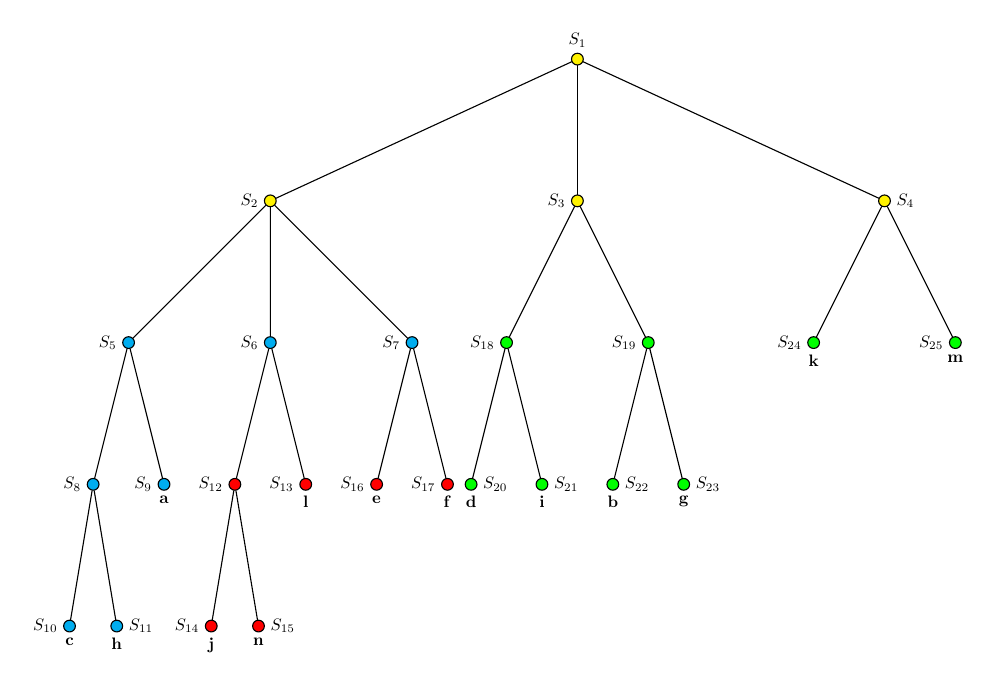
\begin{tikzpicture}[scale=0.6, every node/.style={scale=0.6}]
 
              \node[solid node, label=above:{$S_{1}$}]{}
                child{node[solid node, label=left:{$S_{2}$}]{}
                  child{node(l1)[blue node, label=left:{$S_{5}$}]{}
                    child{node[blue node, label=left:{$S_{8}$}]{}
                      child{node[blue node, label=below:{$\mathbf{c}$}, label=left:{$S_{10}$}]{}
                        edge from parent node{}}
                      child{node[blue node, label=below:{$\mathbf{h}$}, label=right:{$S_{11}$}]{}
                        edge from parent node{}}
                      edge from parent node{}}
                    child{node[blue node, label=below:{$\mathbf{a}$}, label=left:{$S_{9}$}]{}
                      edge from parent node{}}
                    edge from parent node{}
                  }
                  child{node(l2)[blue node, label=left:{$S_{6}$}]{}
                    child{node[red node, label=left:{$S_{12}$}]{}
                      child{node[red node, label=below:{$\mathbf{j}$}, label=left:{$S_{14}$}]{}
                        edge from parent node{}}
                      child{node[red node, label=below:{$\mathbf{n}$}, label=right:{$S_{15}$}]{}
                        edge from parent node{}}
                      edge from parent node{}}
                    child{node[red node, label=below:{$\mathbf{l}$}, label=left:{$S_{13}$}]{}
                      edge from parent node{}}
                    edge from parent node{}
                  }
                  child{node(l3)[blue node, label=left:{$S_{7}$}]{}
                    child{node[red node, label=below:{$\mathbf{e}$}, label=left:{$S_{16}$}]{}
                      edge from parent node{}}
                    child{node[red node, label=below:{$\mathbf{f}$}, label=left:{$S_{17}$}]{}
                      edge from parent node{}}
                    edge from parent node{}
                  }
                  edge from parent node{}
                }
                child{node[solid node, label=left:{$S_{3}$}]{}
                  child{node(l1)[green node, label=left:{$S_{18}$}]{}
                    child{node[green node, label=below:{$\mathbf{d}$}, label=right:{$S_{20}$}]{}
                      edge from parent node{}}
                    child{node[green node, label=below:{$\mathbf{i}$}, label=right:{$S_{21}$}]{}
                      edge from parent node{}}
                    edge from parent node{}
                  }
                  child{node(l2)[green node, label=left:{$S_{19}$}]{}
                    child{node[green node, label=below:{$\mathbf{b}$}, label=right:{$S_{22}$}]{}
                      edge from parent node{}}
                    child{node[green node, label=below:{$\mathbf{g}$}, label=right:{$S_{23}$}]{}
                      edge from parent node{}}
                    edge from parent node{}
                  }
                  edge from parent node{}
                }
                child{node[solid node, label=right:{$S_{4}$}]{}
                  child{node(r1)[green node, label=below:{$\mathbf{k}$}, label=left:{$S_{24}$}]{}
                    edge from parent node{}
                  }
                  child{node(r2)[green node, label=below:{$\mathbf{m}$}, label=left:{$S_{25}$}]{}
                    edge from parent node{}
                  }
                  edge from parent node{}
                }
              ;
            
          \end{tikzpicture}
          \end{center}
          \end{figure}
          
         % Written explanation
	Firstly, we shall label each constraint such that they can subsequently be referred to by index only:
	
	\begin{multicols}{4}
		\begin{enumerate}
			\item $(e, f) < (k, d)$
			\item $(c, h) < (a, n)$
			\item $(j, n) < (j, l)$
			\item $(c, a) < (f, h)$
			\item $(j, l) < (e, n)$
			\item $(n, l) < (a, f)$
			\item $(d, i) < (k, n)$
			\item $(d, i) < (g, i)$
			\item $(c, l) < (g, k)$
			\item $(g, b) < (g, i)$
			\item $(g, i) < (d, m)$
			\item $(c, h) < (c, a)$
			\item $(e, f) < (h, l)$
			\item $(j, l) < (j, a)$
			\item $(k, m) < (e, i)$
			\item $(j, n) < (j, f)$
		\end{enumerate}
	\end{multicols}
	
	The initial inputs into the top layer of recursion are the set of nodes $S = \{a, b, \ldots, n\}$ and the set of constraints $C = \{1, 2, \ldots, 16\}$. We will refer to these as $S_{1}$ and $C_{1}$. The first partition we compute is $\pi_{C_{1}}$. Following the fist condition outlined in Section \ref{section:2A} and detailed in Algorithm \ref{alg:partition} lines 5--18, we generate the initial partition sets $\pi_{C_{1}} = \{e, f\}, \{c, h, a, j, n, l\}, \{d, i, g, b\}, \{k, m\}$. The second condition (lines 23--26) means we must compute merges, generating the partition $\pi_{C_{1}} = \{a, c, e, f, h, j, l, n\}, \{b, d, g, i\}, \{k, m\}$. We will denote these subsets $S_{2}, S_{3}$, and $S_{4}$. This process is shown through the yellow nodes in Figure \ref{fig:tree1}.
	
	Now we recurse into the subset $S_{2} = \{a, c, e, f, h, j, l, n\}$ with the corresponding constraints subset $C_{2} = \{2, 3, 4, 5, 6, 12, 13, 14, 16\}$, applying $BUILD(S_{2}, C_{2})$. This recursive step produces the partition $\pi_{C_{2}} = \{a, c, h\}, \{j, l, n\}, \{e, f\}$. We will denote these as $S_{5}, S_{6}$, and $S_{7}$. Next we recurse further into $S_{5} = \{a, c, h\}$ with $C_{5} = \{12\}$. This generates the partition $\pi_{C_{5}} = \{c, h\}, \{a\} = S_{8}, S_{9}$. When recursing into $S_{8}$ we find $C_{8} = \emptyset$ and so output the partition $\pi_{C_{8}} = \{c\}, \{h\} = S_{10}, S_{11}$, thus meaning the nodes $c$ and $h$ are the leftmost deepest leaves. We can also see that $S_{9}$ is a singleton set, and is thus the leaf node $a$ at the above level of recursion. This is visualised through the blue nodes in Figure \ref{fig:tree2}.
	
	As we go up the levels of recursion, we next need to compute $BUILD(S_{6}, C_{6})$ where $S_{6} = \{j, l, n\}$ and $C_{6} = \{6\}$ to generate the partition $\pi_{C_{6}} = \{j, n\}, \{l\} = S_{12}, S_{13}$. We first recurse into $BUILD(S_{12}, C_{12})$, where $C_{12} = \emptyset$, resulting in two singleton sets $S_{14}$ and $S_{15}$ indicating $j$ and $n$ are leaves at this level. On observation of the singleton set $S_{13}$ at the level above we find that $l$ is a leaf here. The next lowest recursion, $BUILD(S_{7} = \{e, f\}, C_{7} = \emptyset)$, gives the singleton sets $S_{16} = \{e\}$ and $S_{17} = \{f\}$, indicating $e$ and $f$ are leaves at this level. Figure \ref{fig:tree3} demonstrates this process through the red nodes.
	
	Next we recurse back to the top level, applying $BUILD(S_{3} = \{b, d, g, i\}, C_{3} = \{8, 10\})$, to generate the partition $\pi_{C_{3}} = \{d, i\}, \{b, g\} = S_{18}, S_{19}$. Recursing upon the first set of this partition, $BUILD(S_{18}, C_{18} = \emptyset)$, gives the partition $\pi_{C_{18}} = \{d\}, \{i\} = S_{20}, S_{21}$ and thus leaves $d$ and $i$ at this level. Similarly, $BUILD(S_{19}, C_{19} = \emptyset)$ gives $\pi_{C_{19}} = \{b\}, \{g\} = S_{22}, S_{23}$ and leaves $b$ and $g$. Once again, we return to the top level of recursion and compute $BUILD(S_{4} = \{k, m\}, C_{4} = \emptyset)$, giving the partition $\pi_{C_{C_{4}}} = \{k\}, \{m\} = S_{24}, S_{25}$, which when we recurse into give the final two leaves $k$ and $m$. This concludes the algorithm, and thus the full tree is output, shown through in Figure \ref{fig:tree4} (the green nodes indicating the additions from this part).
	
	\subsection{Part D}
	\label{section:2D}
	\subsubsection{\emph{Reverse-BUILD} Algorithm Implementation}
	
	\begin{algorithm}
		\caption{Reverse-BUILD}
		\label{alg:reverse}
		\textbf{Input:} tree $T$ with labelled leaves $S$ \\
		\textbf{Output:} a corresponding the set of constraints $C$
		
		\begin{algorithmic}[1]
			\STATE initialise $C \leftarrow \emptyset$
			
			\FORALL{non-root layers $L_{i}$ of $T$ (from deepest leaves to the layer before the root)}
				
				\STATE assign each leaf $l$ at layer $L_{i}$ the singleton set containing its value $S_{l} = \{v_{l}\}$
				
				\FORALL{non-leaf nodes $p$ in layer $L_{i + 1}$ (above $L_{i}$)}
					
					\STATE form the partition $\pi_{p} = S_{1}, S_{2}, \ldots, S_{N}$ consisting of the sets assigned to each of the $N$ children of $p$
					
					\FORALL{sets $S_{m} \in \pi_{p}$ containing more than one element}
						
						\FORALL{other sets $S_{n} \in \pi_{p} \setminus S_{m}$}
							
							\IF{no constraint $(a, b) < (c, d) \in C$ exists where $a, b \in S_{m}$ and either $c \in S_{n}$ or $d \in S_{n}$}
								\STATE sample two distinct leaves from the first set $a, b \in S_{m}$
								\STATE set $c$ equal to either of these leaves $a$ or $b$
								\STATE sample another leaf from the second set set $d \in S_{n}$
								\STATE add a new constraint over these values: $C \leftarrow (a, b) < (c, d)$
							\ENDIF
							
						\ENDFOR
						
						\STATE merge the sets of $\pi_{p}$ and assign this to the corresponding parent node $p$
					\ENDFOR
				\ENDFOR
			\ENDFOR
			\RETURN the set of constraints $C$
	\end{algorithmic}
	\end{algorithm}
	
	The proposed algorithm \emph{Reverse-BUILD} is shown through the pseudocode in Algorithm \ref{alg:reverse}. It implements an iterative method for building a set of constrains $C$ from a given tree $T$ through which we could apply the $BUILD$ algorithm and construct a tree isomorphic to $T$. This is done through splitting $T$ into distinct layers, where each layer contains all nodes at the same depth, and considering each of these layers $L_{i}$ through a bottom-up approach. We start at the deepest layer and assign each of the leaves its own singleton set; sets on sibling leaves are then merged and assigned to label the corresponding parent node $p$.
	
	We then consider the next layer, where similarly any leaves are assigned to singleton sets. Then, we construct a partition over all sibling nodes in layer $L_{i}$ (with the same parent $p$ in layer $L_{i + 1}$), consisting of the sets associated with each child (if a child is a leaf the associated set will be a singleton set). Namely, for the parent node $p$ in layer $L_{i + 1}$ with $N$ children in layer $L_{i}$, the following partition is constructed over the sets $S_{1} \to S_{N}$ of the children $1 \to N$ of $p$: $\pi_{p} = S_{1}, S_{2}, \dots, S_{N}$. For each set $S_{m} \in \pi_{p}$, we then loop over all other sets $S_{n}$ in the same partition and ensure there is a constraint which links the elements of $S_{m}$ and $S_{n}$, following the two constraint rules described in Section \ref{section:2A}.
	
	The construction of this constraint (in absence of one existing already) is implemented through the lines 8--13 in Algorithm \ref{alg:reverse}, which is done adhering to both rules. We need to ensure this is the case between every set in the partition so that the correct dependencies between nodes are exhibited in the full constraint set. If this is followed, it maintains that when the $BUILD$ algorithm is applied to the full set we can once again generate the same partitions (when we reach this level of the tree).
	
	Once we have ensured all pairs of sets in $\pi_{p}$ have a corresponding constraint in $C$ satisfying the aforementioned rules, all sets in the partition are merged into a single superset containing all values within partition. This set is then linked to the node $p$ such that upon the next iteration, when we are considering the nodes on its level to construct the partition, this set will be used as the set $S_{p}$ associated with node $p$. After this has been performed for all collections of siblings in level $L_{i}$ (i.e. for all parents in $L_{i + 1}$), we move up to layer $L_{i + 1}$ and repeat.
	
	\subsubsection{Proof of Correctness}
	
	For the base case of \emph{Reverse-BUILD}, we have the leaves $a$ and $b$, which will be given the singleton sets $\left\{v_{a}\right\}$ and $\left\{v_{b}\right\}$. As these do not have more than one element, no constraint is constructed and we merge them into a set of two at their parent $c$. When we arrive back to node $c$ during the forward \emph{BUILD} algorithm, and wish to construct the partition of the set $\left\{v_{a}, v_{b}\right\}$, these nodes will be split into two singleton leaf nodes holding each value (as the set is of length 2 and thus can wholly contain no constraints). Thus, for leaves, the same tree structure is maintained over the forward and backwards passes.
	
	Next, consider the case further into the application of \emph{Reverse-BUILD}, where we are considering the parent node $f$, where we constructed the partition $\pi_{f} = \left\{v_{a}, v_{b}\right\},  \left\{v_{d}, v_{e}\right\}$ (by collating the sets of the children of $f$). It is clear that upon application of the forwards \emph{BUILD}, for the constructed tree to split in this manner (i.e. produce the two children linked to these sets), there must be a constraint which requires this. Namely, there must be some constraint $(w, x) < (y, z)$ where $w$ and $x$ are distinct nodes in the same set (following the first rule) and $y$ and $z$ are in different sets (second rule). Thus, the constraint set must contain both $(v_{a}, v_{b}) < (v_{a}~\text{or}~v_{b},~v_{c}~\text{or}~v_{d})$ and $(v_{c}, v_{d}) < (v_{c}~\text{or}~v_{d},~v_{a}~\text{or}~v_{b})$. This is implemented through lines 8--13 of Algorithm \ref{alg:reverse}, which arbitrarily selects the first set being considered to take the first two values $(w, x)$, samples one of these for position $y$, and a value from the second set for position $z$. This preserves the presence of a constraint in C such that when the forwards \emph{BUILD} algorithm is applied, the partition splits the total set of values splits into the correct subsets to propagate into each subtree of the current node, maintaining the same overall structure. Specifically, upon the partition $\pi_{f} = \left\{v_{a}, v_{b}\right\},  \left\{v_{d}, v_{e}\right\}$, the algorithm \emph{Reverse-BUILD} would construct constraints analogous to $(v_{a}, v_{b}) < (v_{a}, v_{c})$ and $(v_{c}, v_{d}) < (v_{c}, v_{a})$ (as all pairs of sets in the partition are looped through). The two sets would then be merged into the superset $\left\{v_{a}, v_{b}, v_{c}, v_{d}\right\}$ at their parent. When this parent is considered whilst applying the forwards \emph{BUILD}, we will be tasked with generating a partition over the set $\left\{v_{a}, v_{b}, v_{c}, v_{d}\right\}$. Because the constraint set contains both $(v_{a}, v_{b}) < (v_{a}, v_{c})$ and $(v_{c}, v_{d}) < (v_{c}, v_{a})$, we know $v_{a}, v_{b}$ must be in the same set,  $v_{c}, v_{d}$ must be in the same set, and $v_{a}, v_{c}$ must be in different sets. Hence, the only way these values can be split is through the partition $\left\{v_{a}, v_{b}\right\},  \left\{v_{d}, v_{e}\right\}$, propagating the same sets of values into the subtrees as seen in the original tree (upon which we applied \emph{Reverse-BUILD}).
	
	If this is repeated on every node (for each partition), from the bottom of the tree upwards, this ensures that when that node is being considered during the application of \emph{BUILD}, the same partitions are constructed, and thus the same values are propagated into each subtree, resulting in the same overall tree structure. Additionally, further into the application of \emph{Reverse-BUILD}, as we consider nodes further up the tree, the partition sets get bigger and bigger. Thus, the likelihood that, when we are considering two sets $X$ and $Y$ in said partition, a constraint will exist between these two sets increases, and so the number of constraints that have to be constructed at every node decreases over the algorithmic process. Hence, only the necessary amount of constrains are added to the set to reconstruct the tree structure exactly, and if a constraint exists which already fulfils this criteria then redundant constraints are not further added (which would overfill the total constraint set).
		
\end{document}
